\section{Data} \label{Data}
The data presented in the following and was used to calibrate the disaster risk model has been taken from \citet{Jorda2017}, who ``painstakingly compiled annual asset return data for 16 advanced countries, over nearly 150 years.'' A current version of the public data set may be found on \textcolor{blue}{\href{http://www.macrohistory.net/data/}{Jordà-Schularick-Taylor Macrohistory Database}} (http://www.macrohistory.net/data/). Moreover, the authors acknowledge the ``largest but often ignored component of household wealth, housing'' and provide total returns data, including housing. Although this component does certainly constitute a capital asset with its own, very specific characteristics affecting the households' consumption-savings decision I will omit it and focus on stock market returns (i.e. out of risky assets) for comparability across countries and the existing literature.

For convenience and familiarisation with the data set I found it useful to develop an own \textcolor{blue}{\href{http://disaster-app-master.herokuapp.com/}{web application}} (http://disaster-app-master.herokuapp.com/) in Python using Dash\footnote{https://plotly.com/dash/, a HTML wrapper framework for building analytical web apps, mainly used in Machine Learning and Data Science drawing from interactive Plotly graphics} for visualisation and exploration. The GitHub repository may be found \textcolor{blue}{\href{https://github.com/gerwolf/macro-disaster}{here}} https://github.com/gerwolf/macro-disaster.

Some corrections had to be applied, in particular for stock market data in Germany during the period of hyperinflation (1914-1924) where outliers were removed and imputed using the real performance index by \citet{Gielen1994} which had a Pearson correlation coefficient of about 0.8 with the Jordà-Schularick-Taylor (JST) measure of real total return on equity between the years 1872 and 1992 excluding the years 1922-1924. Other missing values were imputed using moving averages.

Table \ref{tab:data_coverage} in the appendix describes the availability for each key series, earliest starting in 1870 and in unbalanced cases starting dates were chosen such that they were no different within countries, except for Belgium, Japan and Portugal due to missing consumption data but otherwise complete series.

Altogether, the sample accounts for about 35\% of the world GDP in 2015 (PPP) according to the World Bank database\footnote{Accessed 13/09/2020}. The relative composition inside the sample \footnote{measured in real GDP (PPP) using the Maddison Project dataset}, however, did change considerably between 1900 and 2015. The US increased their contribution from 30\% to 47\% whereas the UK's share decreased by 11\% to 7\% followed by Germany with a reduction of 8\% to 8\%. Japan increased it's proportionate contribution from 5\% to 13\%. At the global level returns and growth data are considered from 1900 to 2015 due to incompleteness of observations and weightings before that date.

\subsection{International financial markets}
Total nominal (gross) returns for asset $i$ in country $j$ at time $t$ were calculated according to
\begin{align*}
    R_{i,j,t} &= \frac{P_{i,j,t} - P_{i,j,t-1}}{P_{i,j,t-1}} + Y_{i,j,t}
\end{align*}
where $P$ is the asset's price and $Y$ is the yield component, e.g. dividends. Total real (net) returns were calculated according to
\begin{align*}
    r_{i,j,t} &= \frac{1+R_{i,j,t}}{1+\pi_{j,t}} - 1
\end{align*}
where $\pi$ is the inflation rate.\\
\\
At the global level (see table \ref{tab:global_returns}), i.e. equally weighted as well as real GDP-value weighted average rates of return, real rates of return on equity outperformed Treasury bills with 6.57\% (7.03\%) equally weighted (real-GDP weighted) compared to -0.39\% (-0.17\%) resulting in an equity risk premium of 6.96\% (7.20\%). Variability was higher for equity than for relatively safe assets by a factor of 3.

{\renewcommand{\arraystretch}{1}
\begin{table}[H]
\begin{center}
\begin{tabular}{rccccccc}
\hline
\hline
 & \multicolumn{3}{c}{All equally weighted} & & \multicolumn{3}{c}{real GDP-weighted} \\
 \cline{2-4} \cline{6-8}
 & Equity & Bills & ERP & &Equity & Bills & ERP \\
\hline
Full sample & & & & & & & \\
\hline

Mean return p.a. & 6.57 & -0.39 & 6.96 & & 7.03 & -0.17 & 7.20\\ 

Std. dev. & 15.43 & 6.28 & 14.66 & & 15.26 & 5.95 & 15.02\\ 

Geometric mean & 5.37 & -0.61 & 5.88 & & 5.86 & -0.36 & 6.07\\ 

Median & 6.68 & 1.07 & 6.97 & & 7.46 & 1.39 & 8.27\\ 

Max & 39.45 & 10.84 & 36.57 & & 48.34 & 11.94 & 47.28\\ 

Min & -46.09 & -28.83 & -46.42 & & -41.38 & -21.44 & -41.20\\ 

Kurtosis & 3.87 & 7.95 & -4.08 & & 3.61 & 6.64 & 3.82\\ 

\hline 
Post-1984 & & & & & & & \\
\hline 

Mean return p.a. & 10.89 & 2.22 & 8.67 & & 9.31 & 1.93 & 7.37\\ 

Std. dev. & 20.39 & 2.34 & 20.27 & & 16.86 & 2.16 & 16.58\\ 

Geometric mean & 8.77 & 2.20 & 6.54 & & 7.84 & 1.91 & 5.94\\ 

Median & 12.02 & 2.15 & 12.14 & & 13.26 & 2.37 & 13.00\\ 

Max & 39.45 & 5.83 & 35.28 & & 33.81 & 5.11 & 32.52\\ 

Min & -46.09 & -1.23 & -46.42 & & -41.38 & -1.83 & -41.20\\ 

Kurtosis & 3.65 & 1.74 & 3.38 & & 4.44 & 1.76 & 4.17\\ 
\hline
\hline
\end{tabular} 
\end{center}
\caption{Global real returns (1900-2015)}
\label{tab:global_returns}
\end{table}

For the post-1984 period subset returns across both asset classes were higher compared to the full sample
%with an unweighted (real-GDP weighted), annual mean return of 10.89\% (9.31\%) for equity and 2.22\% (1.93\%) for Treasury bills. 
Volatility was higher in this period for equity but smaller for T-bills. %Note that the biggest stock market turmoils out of the entire sample occured in the post-1984 period whereas Treasury bills remained stable during that period. Overall, the ERP was 8.67\% in the unweighted sample and 7.37\% in the real-GDP weighted sample.


\begin{figure}[H]
	\begin{tabular}{cc}
	\subfloat[Equity]{
		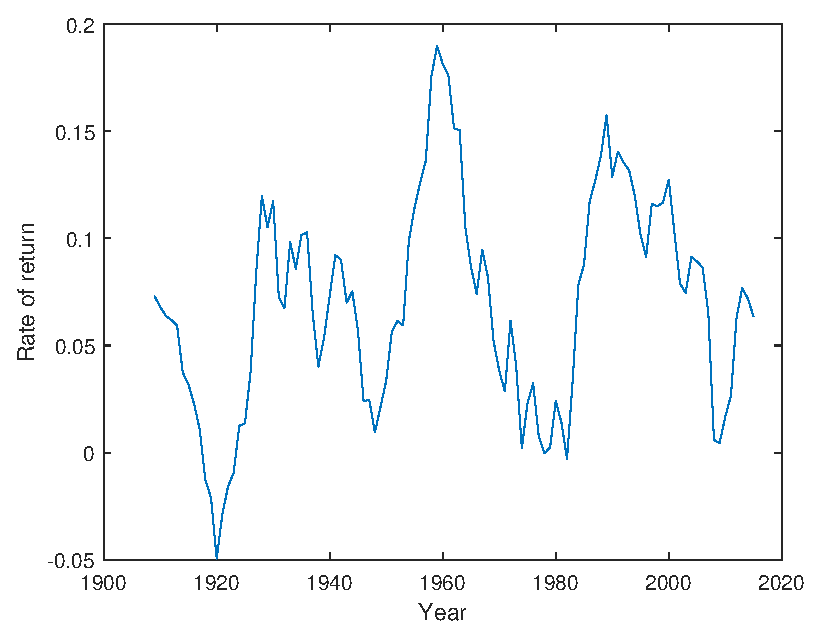
\includegraphics[keepaspectratio = true, width = 0.45\textwidth]{Matlab Graphics/Figure_2_equity}
	} &
	\subfloat[Treasury bills]{
		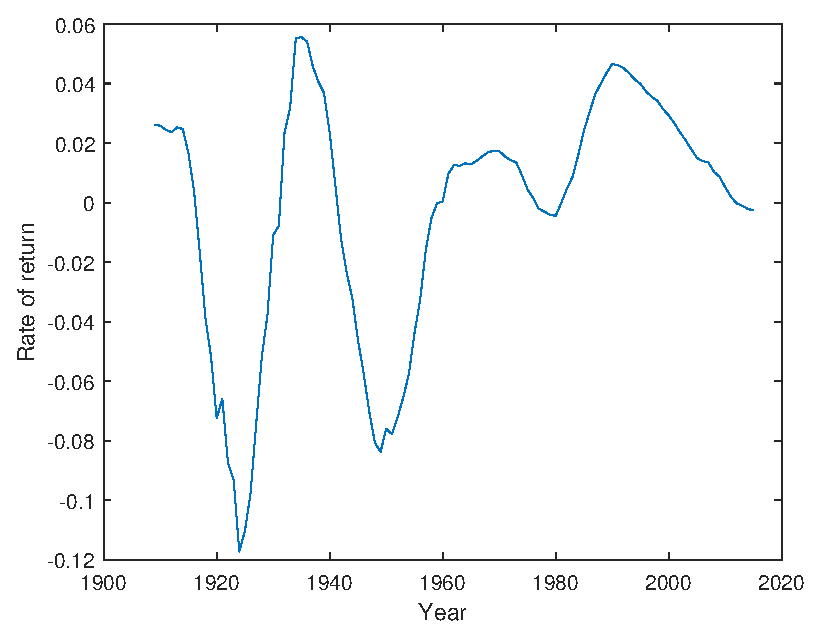
\includegraphics[width = 0.45\textwidth]{Matlab Graphics/Figure_2_bills}
	}\\
	\end{tabular}
	\caption{Decadal, real-GDP weighted moving averages of asset returns}
	\label{fig:decadal_MA_asset_returns}
\end{figure}

Figure \ref{fig:decadal_MA_asset_returns} indicates that returns on equity and T-bills show some cyclical behaviour with equity being more volatile than risk-free rates.\\
\\
At the country-level (see table \ref{tab:real_returns_countries} in the appendix) there is some degree of variation in asset returns; returns on equity range from values as low as 3.02\% (France) to 8.90\% (Finland). Treasury bills returned, on average, -2.57\% (Germany) to 2.99\% (Denmark). Interestingly, German investors lost on average 2.57\% of their initial wealth when holding safe assets \footnote{\citet{Probst2019} estimates the average short-term real interest rate for Germany (1871-2013) even lower at -3.5\%.}. German \textit{Bunds} are recognized as one of the assets with the lowest probability of default, hence making it a valuable asset as it provides (almost) perfect insurance, driving up its price and lowering its return. In total, for seven countries the measured average real risk-free rate was negative.% Similarly to global rates, asset returns were higher during the post-1984 period than in the entire sample period with higher associated volatility, though. 
\newpage
The resulting premiums are documented in table \ref{tab:erp_countries} below:

{\renewcommand{\arraystretch}{1}
\begin{table}[H]
\begin{center}
\begin{tabular}{rccccc}
\hline
\hline
Country & \multicolumn{2}{c}{Full sample (1870-2015)} & & \multicolumn{2}{c}{post-1984} \\
\cline{2-3} \cline{5-6}
& Mean & Std & & Mean & Std\\
\hline
Australia & 6.59 & 15.86 & & 5.13 & 18.76\\
Belgium & 5.91 & 22.89 & & 9.68 & 24.85\\
Denmark & 4.90 & 18.01 & & 8.15 & 22.72\\
Finland & 10.34 & 30.90 & & 12.90 & 42.40\\
France & 4.34 & 21.37 & & 8.02 & 24.45\\
Germany & 10.47 & 36.62 & & 8.50 & 24.96\\
Italy & 6.50 & 30.81 & & 7.09 & 29.80\\
Japan & 9.24 & 27.00 & & 4.20 & 22.56\\
Netherlands & 6.51 & 23.08 & & 8.66 & 22.80\\
Norway & 5.00 & 20.36 & & 10.36 & 29.24\\
Portugal & 4.14 & 27.45 & & 9.44 & 39.37\\
Spain & 6.37 & 21.30 & & 11.84 & 28.31\\
Sweden & 6.45 & 20.00 & & 11.75 & 28.10\\
Switzerland & 5.76 & 18.73 & & 9.39 & 22.51\\
United Kingdom & 5.94 & 19.24 & & 5.75 & 15.45\\
United States & 6.28 & 18.36 & & 7.92 & 16.44\\
\hline
\hline
\end{tabular} 
\end{center}
\caption{Equity risk premium (country-level), \%}
\label{tab:erp_countries}
\end{table}

%The highest risk premium was 10.47\% for Germany, the lowest was 4.14\% for Portugal in the full sample. The global, unweighted ERP was about 6.55\% in the full sample and 8.67\% for the post-1984 period. 
%Variability in the market price of risk did also increase in the post-1984 period, indicating more frequently fluctuating consumption according to the theoretical models described in section \ref{introduction}.
Measuring the intra-sample consistency (by the standardized coefficient of variation across countries) in risk-free rates shows an interesting picture how stable they really were in the past:

\begin{figure}[H]
	\begin{tabular}{cc}
	\subfloat[1900-1983]{
		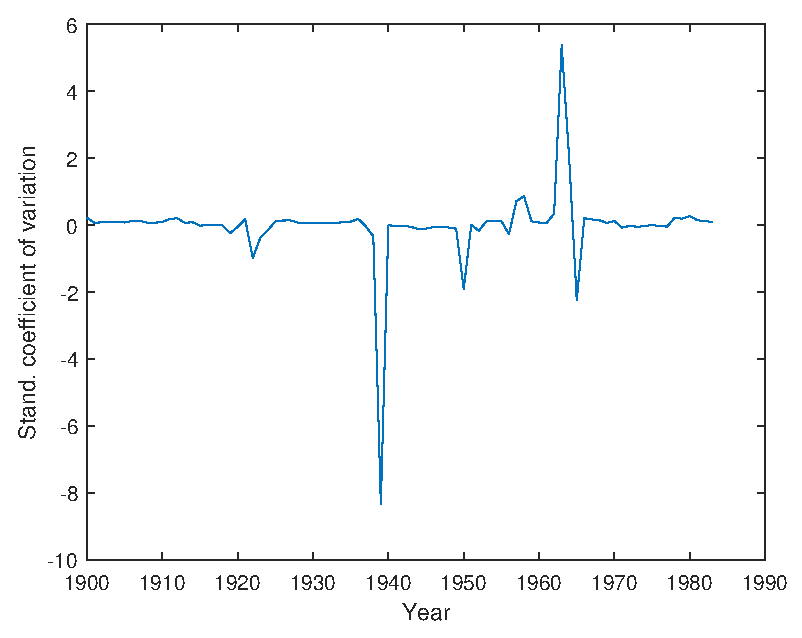
\includegraphics[width = 0.45\textwidth]{Matlab Graphics/Figure_3_1900_1983}
	} &
	\subfloat[Post-1984]{
		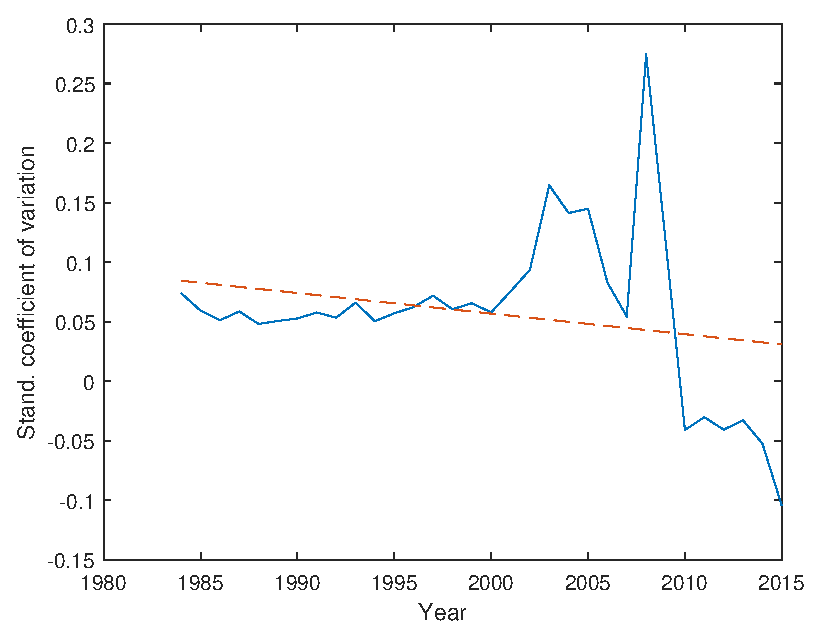
\includegraphics[width = 0.45\textwidth]{Matlab Graphics/Figure_3_1984_2015}
	}\\
	\end{tabular}
	\caption{Standardized coefficient of variation (risk-free rate)}
	\label{fig:stand_coeff_var_riskfree}
\end{figure}

%Major economic shocks such as wartime but also the 1960s posed disturbances to the capital market. Most of the time, however, risk-free rates were rather stable within and across countries. 
The right panel of figure \ref{fig:stand_coeff_var_riskfree} shows a period of global calmness interrupted by the Dot-com bubble and the 2008 financial crisis. Since then risk-free rates entered negative terrain, although monetary authorities' responses were quite consistent in this regard.
Using cross-sectional aggregates it is noteworthy to highlight the two different asset classes' characteristics with respect to ``risk'' and expected return.

\begin{figure}[H]
	\centering
  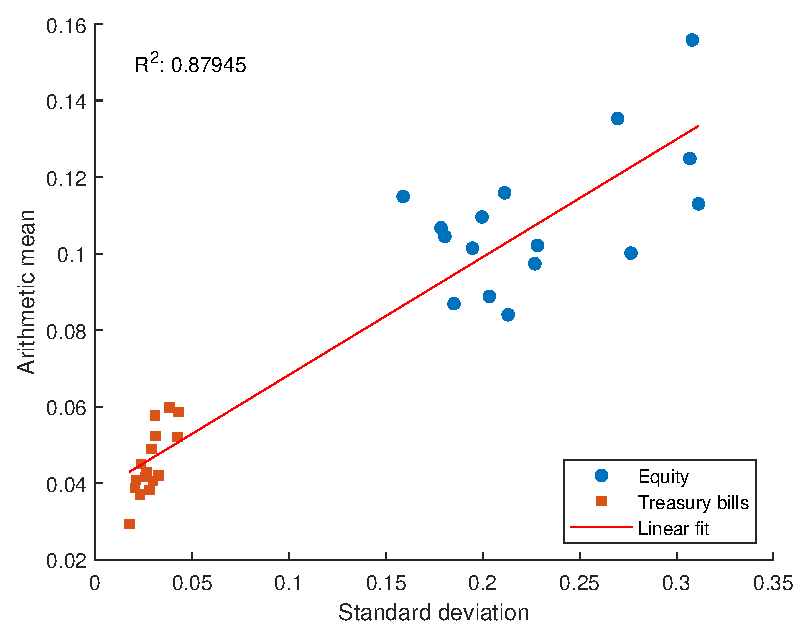
\includegraphics[width=0.7\textwidth]{Matlab Graphics/Figure_4_capital_market_line}
	\caption{Capital market line}
	\label{fig:cml}
\end{figure}

The capital market line (figure \ref{fig:cml}) plots the arithmetic mean of nominal returns against the volatility, measured as the standard deviation of these returns for the two asset classes. Clearly, there is a positive relationship between expected return and volatility within the asset classes but also across them, as confirmed by a formal Chow-test for structural differences between these two classes. Adding an intercept for each class does not improve the goodness of fit (F-distributed Chow-test statistic: 5.42 $<$ critical value with $k=2$ degrees of freedom in the numerator and $n=28$ degrees of freedom in the denominator at $\alpha$ = 0.05: 8.93), hence there are no structural differences in the risk-return relationship across programmes.\\
\\
Finally, turning to the cross-country equity risk premiums reveals dynamic variation within and across countries (figure \ref{fig:erp_countries_time} below).

\begin{figure}[H]
	\centering
  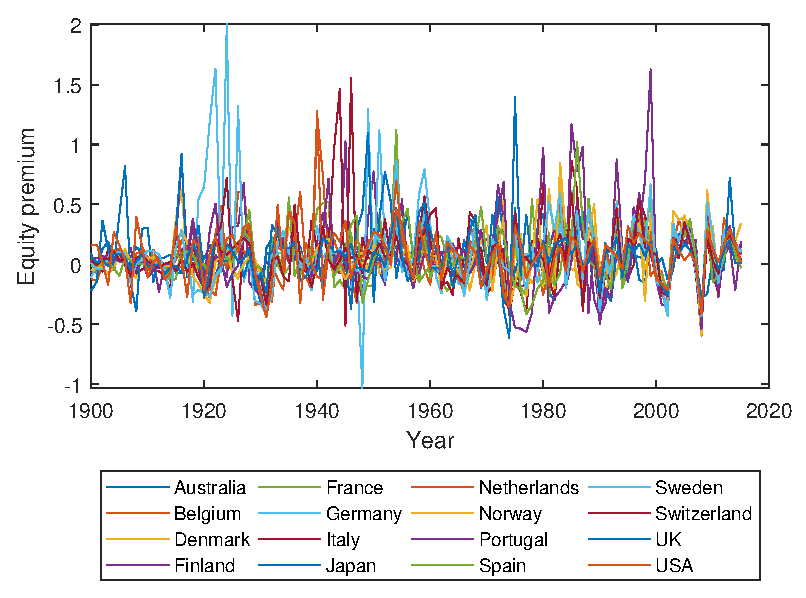
\includegraphics[width=\textwidth]{Matlab Graphics/Figure_5_ERP_countries}
	\caption{Equity risk premiums across countries over time}
	\label{fig:erp_countries_time}
\end{figure}

It appears there is some volatility clustering during wartime across countries but also during prolonged episodes of peace and economic prosperity. The global measure for the equity risk premiums provides more clarity on the dynamic behaviour, that is it's high when there is turmoil and falls as economic conditions improve (see figure \ref{fig:erp_global_time}). 
%A principal component analysis of the ERP cross-country correlations between 1900 and 2015 suggests that one component captures about as much variation as found in six countries (out of sixteen), translating into about 40\% of total variance and appropriately captures within-model (Hotelling's $T^{2}$) and outside-model (squared prediction errors) consistency. Turns out that this component is exactly the negative of the unweighted average. 
%In short, even though cross-country heterogeneity in terms of ERP levels looks pronounced, it actually isn't and only a few exceptional years (see figure \ref{fig:stand_coeff_var_erp}) falling into wartime as well as extraordinary (recovery) growth periods prove the rule. 
Figure \ref{fig:stand_coeff_var_erp} confirms an overall and more recent harmonization \textbf{and} synchronization of equity risk premiums across countries.

\begin{figure}[ht]
	\centering
  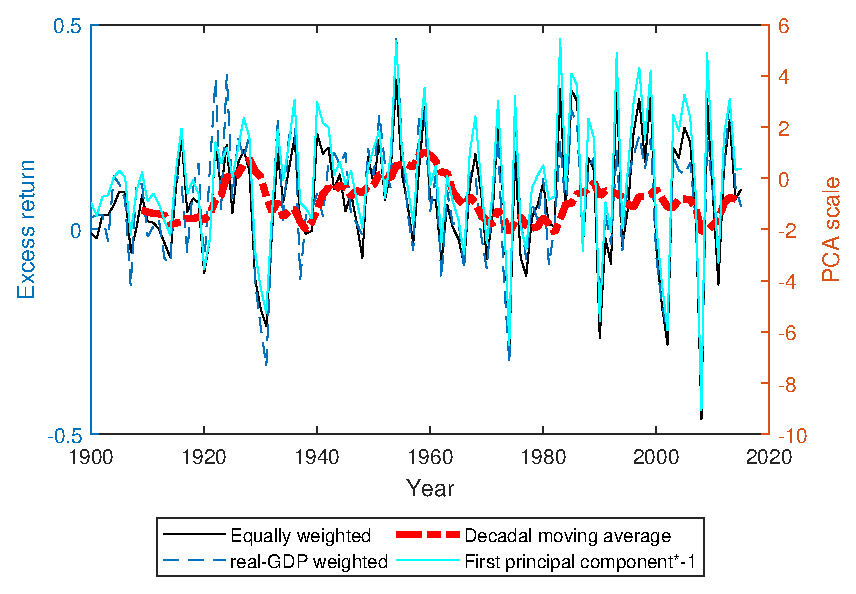
\includegraphics[width=0.8\textwidth]{Matlab Graphics/Figure_6_global_ERP}
	\caption{Global equity risk premium over time}
	\label{fig:erp_global_time}
\end{figure}

\begin{figure}[H]
	\begin{tabular}{cc}
	\subfloat[1900-1983]{
		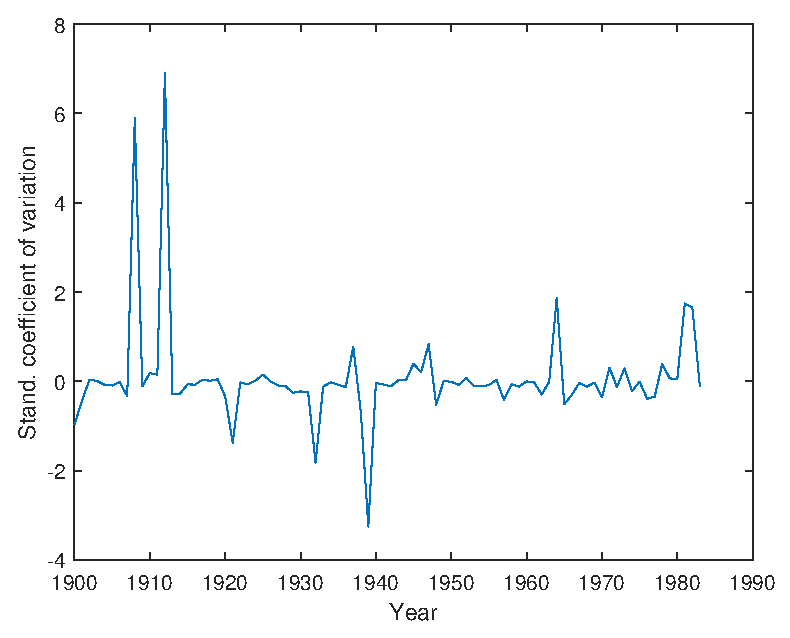
\includegraphics[width = 0.45\textwidth]{Matlab Graphics/Figure_7_1900_1983}
	} &
	\subfloat[Post-1984]{
		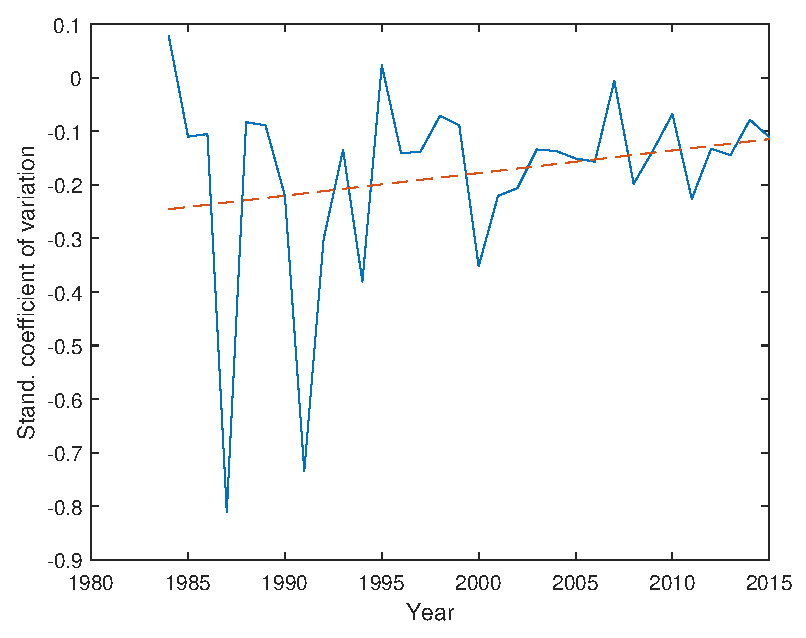
\includegraphics[width = 0.45\textwidth]{Matlab Graphics/Figure_7_1984_2015}
	}\\
	\end{tabular}
	\caption{Standardized coefficient of variation (equity risk premium)}
	\label{fig:stand_coeff_var_erp}
\end{figure}

\newpage
\subsection{International macroeconomic aggregates}
Descriptive statistics for global growth rates are given in table \ref{tab:global_growth} below:

{\renewcommand{\arraystretch}{1.0}
\begin{table}[H]
\begin{center}
\begin{tabular}{rccccc}
\hline
\hline
& \multicolumn{2}{c}{Equally weighted} & & \multicolumn{2}{c}{real GDP-weighted} \\
\cline{2-3} \cline{5-6}
& GDP & consumption & & GDP & consumption\\
\hline
Full sample & & & & &\\
\hline
Mean growth rate p.a. & 2.10 & 1.87 & & 2.14 & 1.81\\
Std.dev. & 2.68 & 2.98 & & 3.12 & 2.53\\
Geometric mean & 2.06 & 1.83 & & 2.09 & 1.78\\
Median & 2.41 & 1.91 & & 2.24 & 2.03\\
Max & 11.10 & 15.17 & & 9.60 & 13.84\\
Min & -6.40 & -6.98 & & -9.41 & -5.28\\
Kurtosis & 5.00 & 8.02 & & 5.15 & 7.45\\
\hline
Post-1984 & & & & &\\
\hline
Mean growth rate p.a. & 1.60 & 1.53 & & 1.67 & 1.71\\
Std.dev. & 1.60 & 1.23 & & 1.54 & 1.18\\
Geometric mean & 1.59 & 1.52 & & 1.66 & 1.71\\
Median & 2.02 & 1.66 & & 1.94 & 1.75\\
Max & 3.66 & 3.60 & & 4.19 & 3.55\\
Min & -4.38 & -1.54 & & -4.20 & -1.45\\
Kurtosis & 7.92 & 2.96 & & 8.99 & 3.52\\
\hline
\hline
\end{tabular} 
\end{center}
\caption{Global growth rates (1900-2015), \%}
\label{tab:global_growth}
\end{table}

As one can see, GDP growth was higher than consumption growth and slightly more volatile. 
%Both macroeconomic aggregate's growth rates are centered around their mean values with rates ranging from -6.98\% to 15.17\% for consumption when all countries were equally weighted and from -9.41\% in GDP to 13.84\% in consumption when countries were real-GDP weighted. 
The post-1984 period is characterised by overall lower growth rates but also volatility where consumption growth is nearly normal distributed. Table \ref{tab:global_growth_HP} in the appendix presents the same statistics for growth rates of the HP-filtered trend component where growth rates are overall lower and also less volatile than the unfiltered data.


Growth rates across countries are presented in table \ref{tab:real_growth_countries} below. 
{\renewcommand{\arraystretch}{1.0}
\begin{table}[H]
\begin{center}
\begin{tabular}{rccccccccccc}
\hline
\hline
Country & \multicolumn{5}{c}{Full sample (1870-2015)} & & \multicolumn{5}{c}{post-1984} \\
%\cline{2-6} \cline{8-12}
\hline
 & \multicolumn{2}{c}{GDP} & & \multicolumn{2}{c}{consumption} & & \multicolumn{2}{c}{GDP} & & \multicolumn{2}{c}{Consumption}\\
\cline{2-3} \cline{5-6} \cline{8-9} \cline{11-12}
 & Mean & Std & & Mean & Std & & Mean & Std & & Mean & Std\\
\hline
Australia & 1.54 & 4.10 & & 1.28 & 5.73 & & 1.91 & 1.47 & & 1.77 & 1.39\\
Belgium$^{*}$ & 1.93 & 8.16 & & 1.73 & 8.64 & & 1.49 & 1.50 & & 1.22 & 1.26 \\
Denmark & 1.76 & 3.66 & & 1.53 & 5.27 & & 1.17 & 1.95 & & 0.93 & 2.40 \\
Finland & 2.18 & 4.50 & & 2.24 & 5.51 & & 1.52 & 3.40 & & 1.84 & 2.82\\
France & 1.85 & 6.25 & & 1.60 & 6.53 & & 1.26 & 1.46 & & 1.25 & 1.18\\
Germany & 2.09 & 7.92 & & 1.84 & 5.54 & & 1.70 & 1.97 & & 1.40 & 1.22\\
Italy & 1.92 & 4.68 & & 1.55 & 3.70 & & 1.37 & 2.60 & & 0.96 & 2.29\\
Japan$^{*}$ & 2.62 & 5.97 & & 2.36 & 6.70 & & 1.55 & 2.23 & & 1.61 & 1.52\\
Netherlands & 1.79 & 7.38 & & 1.76 & 8.32 & & 1.73 & 1.76 & & 1.15 & 1.66 \\
Norway & 2.18 & 3.56 & & 1.92 & 3.71 & & 1.83 & 1.95 & & 2.27 & 2.32\\
Portugal$^{*}$ & 1.95 & 4.25 & & 2.49 & 4.42 & & 1.77 & 2.85 & & 2.31 & 3.21 \\
Spain & 2.00 & 4.90 & & 1.88 &  7.53 & & 2.04 & 2.67 & & 1.55 & 2.71\\
Sweden & 2.10 & 3.39 & & 1.91 & 4.33 & & 1.66 & 2.42 & & 1.35 & 2.03\\
Switzerland & 1.50 & 3.90 & & 1.40 & 6.03 & & 1.03 & 1.69 & & 0.84 & 0.86\\
United Kingdom & 1.45 & 2.87 & & 1.37 & 2.80 & & 1.80 & 1.88 & & 2.10 & 2.25\\
United States & 2.05 & 4.90 & & 1.83 & 3.48 & & 1.73 & 1.75 & & 1.95 & 1.45 \\
\hline
Average & 1.93 & - & & 1.79 & - & & 1.60 & - & & 1.53 & -\\

\hline
\hline
\multicolumn{12}{c}{$^{*}$ Belgium: 1914-2015, Japan: 1875-2015, Portugal: 1911-2015}
\end{tabular} 
\end{center}
\caption{Real growth rates (country-level), \%}
\label{tab:real_growth_countries}
\end{table}

Table \ref{tab:real_growth_countries_HP} in the appendix repeats the same exercise with HP-trend filtered data\footnote{Individual country's indices for real GDP per capita and real consumption expenditures per capita were HP-filtered first and the growth rates of the trend component were then real GDP-weighted.} with overall lower growth rates and lower volatility.

\begin{figure}[H]
	\begin{tabular}{cc}
	\subfloat[Real GDP/capita growth]{
		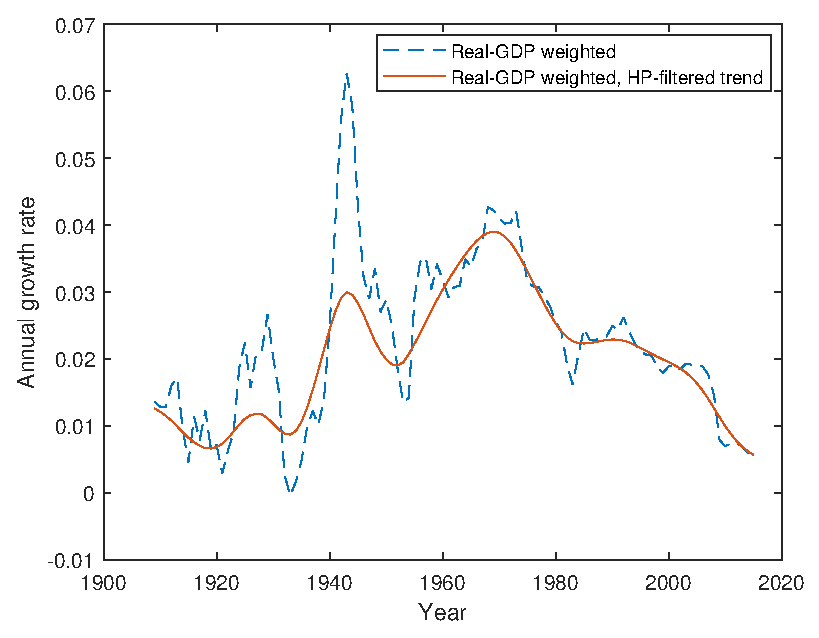
\includegraphics[width = 0.45\textwidth]{Matlab Graphics/Figure_8_GDP}
	} &
	\subfloat[Real consumption/capita growth]{
		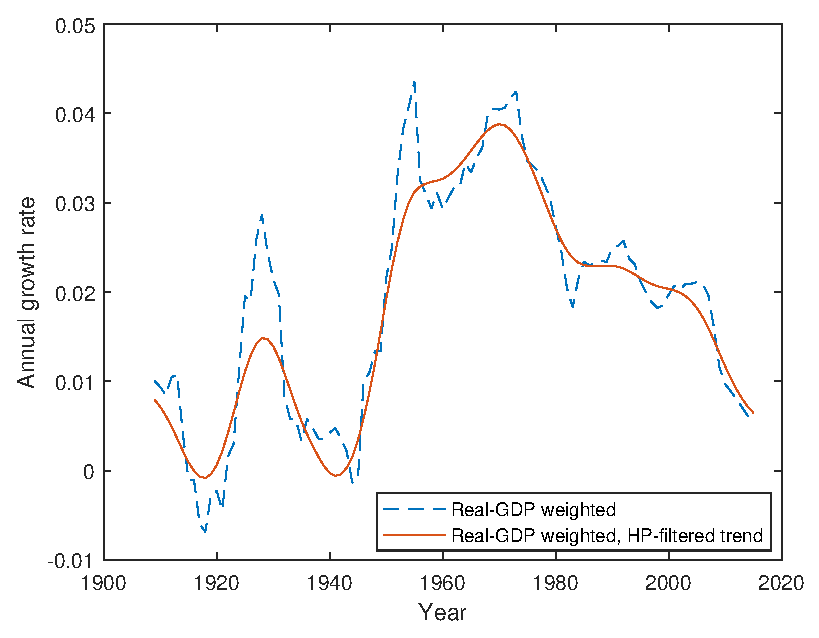
\includegraphics[width = 0.45\textwidth]{Matlab Graphics/Figure_8_cons}
	}\\
	\end{tabular}
	\caption{Decadal moving averages of real-GDP weighted growth rates}
	\label{fig:10y_MA_weighted_growth}
\end{figure}

Figure \ref{fig:10y_MA_weighted_growth} shows the 10-year moving averages for the annual growth rates together with the HP-filtered trend components' growth rates per country, all real-GDP weighted. Since the 1970s both macroeconomic aggregates have been growing at positive but decreasing rates where GDP appears to fluctuate more frequently and variably than consumption. 
Finally, figure \ref{fig:global_business_cycle} displays the real-GDP weighted, HP-filtered countries' trend components growth capturing the world's business cycle dynamics of the last century. Since the 1960s both aggregates move in almost perfect tandem following a downward trend from 4\% annual growth to less than 1\% per year.

\begin{figure}[H]
	\centering
  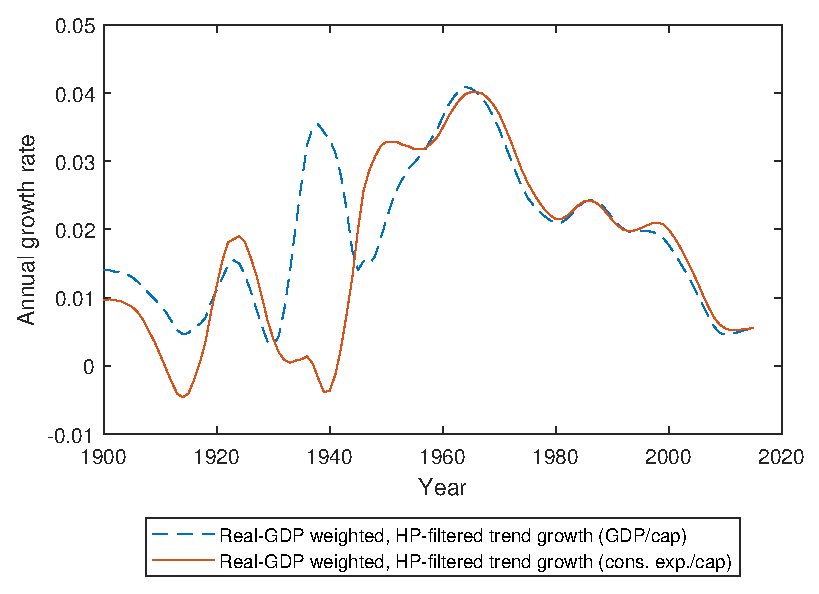
\includegraphics[width=\textwidth]{Matlab Graphics/Figure_9}
	\caption{Global business cycle}
	\label{fig:global_business_cycle}
\end{figure}

\subsection{Macro-finance}
According to \citet{Cochrane2017}, ``Macro-finance studies the relationship between asset prices and economic fluctuations.'' Stock market returns driven by capital gains tend to be high during economic expansions, reflecting higher expected corporate earnings are low during recessions. ``The'' interest rate (solid red line in figure \ref{fig:financial_aggregates_cycles}), however, reflects the opportunity cost of consuming rather than investing and provides a, perhaps the most decisive, incentive to postpone consumption (solid blue line in figure \ref{fig:financial_aggregates_cycles}) when it's high, resulting in lower consumption growth. Figure \ref{fig:financial_aggregates_cycles} below illustrates these relationships of real-GDP weighted returns and growth rates. 
\begin{figure}[ht]
	\centering
  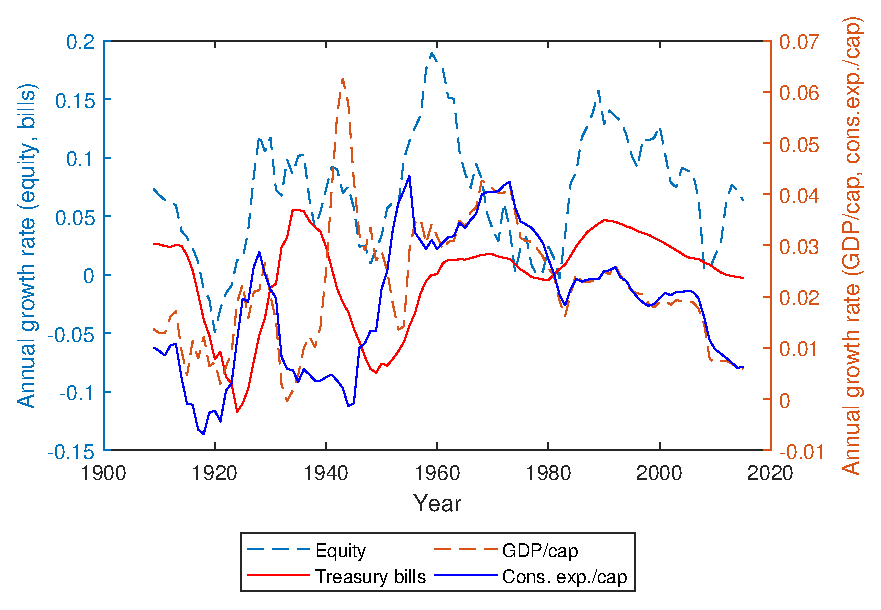
\includegraphics[width=0.8\textwidth]{Matlab Graphics/Figure_10}
	\caption{Financial markets and real economy}
	\label{fig:financial_aggregates_cycles}
\end{figure}
Whereas the first fact, i.e. there is a positive correlation between GDP growth (or consumption growth) and stock market returns ($\rho_{(r^{e}, \Delta GDP)} = 0.23$, $\rho_{(r^{e}, \Delta cons)} = 0.35$) roughly holds over a long horizon the second relationship, i.e. a negative correlation between GDP growth (or consumption growth) and the interest rate appears to have broken down since the 1960s (pre-1965: $\rho_{(r^{f}, \Delta GDP)} = -0.16$, $\rho_{(r^{f}, \Delta cons)} = -0.17$, post-1965: $\rho_{(r^{f}, \Delta GDP)} = 0.09$, $\rho_{(r^{f}, \Delta cons)} = 0.03$). These covariances are exactly the quantities of undiversifyable risk that investors, in theory, are compensated for. The \textit{adequate} magnitude in expectation is the equity risk premium which has been measured in a vast body of literature and applications between 4\% and 8\%.

%Going back to the last relationship between (expected) excess return, risk aversion and variance in consumption growth in subsection \ref{Power utility} clearly illustrates this link. 
For any given level of risk aversion, higher variability in consumption growth (i.e. risk) increases the expected excess return by decreasing the risk-free rate due to the precautionary savings effect. Figure \ref{fig:ERP_riskfree_volatility} below illustrates the theoretical conjectures in the data with the aforementioned divergence starting in the 1980s when global interest rates started to descend.
\begin{figure}[H]
	\begin{tabular}{cc}
	\subfloat[Equity risk premium and consumption volatility]{
		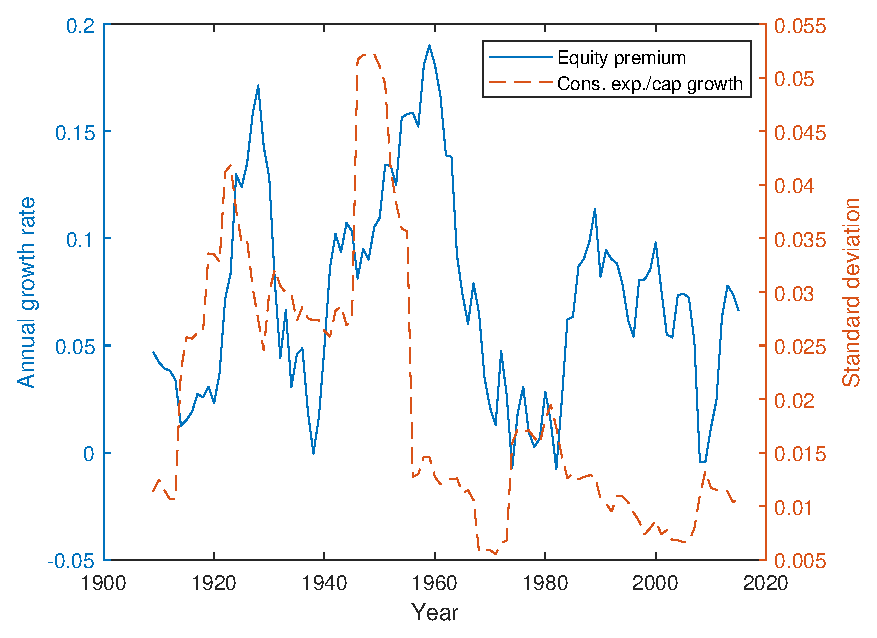
\includegraphics[width = 0.45\textwidth]{Matlab Graphics/Figure_11_ERP}
	} &
	\subfloat[Risk-free rate and consumption volatility]{
		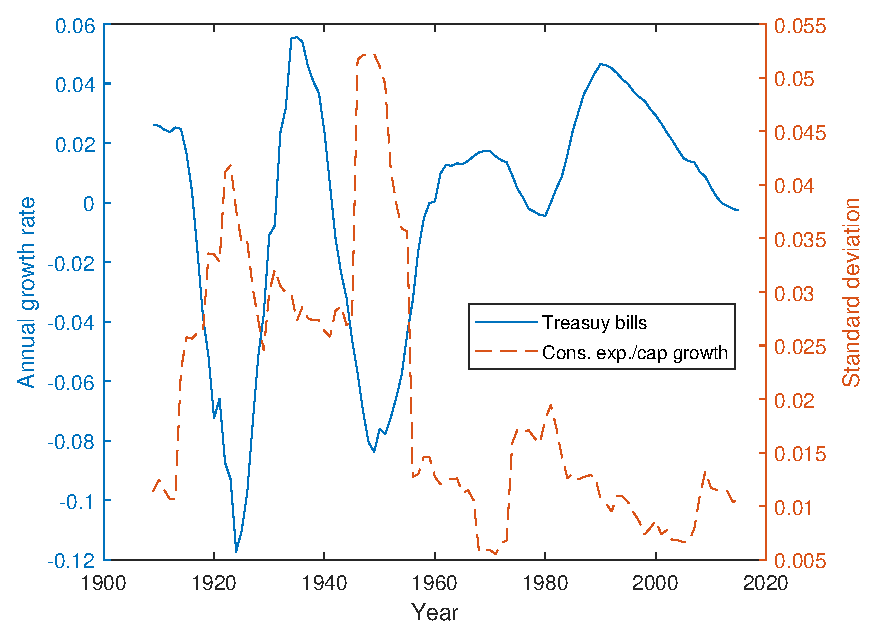
\includegraphics[width = 0.45\textwidth]{Matlab Graphics/Figure_11_riskfree}
	}\\
	\end{tabular}
	\caption{Global decadal moving average of ERP and standard deviation of consumption growth, real-GDP weighted}
	\label{fig:ERP_riskfree_volatility}
\end{figure}
The ERP is positively correlated with the variability in consumption growth (Pearson correlation coefficient of 0.22) whereas the risk-free rate is strongly negatively correlated with variability in consumption growth (Pearson correlation coefficient of -0.73).


With all the ingredients from a (log-normal) consumption-based asset pricing model under time-separable expected utility at hand it is straightforward to derive implied coefficients of relative risk aversion \underline{$\gamma$} (see tables \ref{tab:results_consumption} and \ref{tab:results_GDP} for consumption data and GDP data, respectively for comparison).
%As countries exhibit heterogeneity in risk premiums and consumption growth moments so they do in implied preferences. Most importantly, the implied coefficients of relative risk aversion range from 8 (Belgium) to a whopping 76 (United Kingdom)! 
These are orders of magnitude above the standard evidence for low values of $\gamma$, around 1, coming from the relationship between the risk-free rate and consumption growth which rises quickly in $\gamma$.

\subsection{Disaster empirics}
%What exactly defines an economic disaster? In general, it is a state of very low consumption growth and hence high marginal utility of consumption. Such state must be distinctively different and much more `painful' than normal economic fluctuations which can extend to externality effects such as the destruction of intangible capital. Extreme one-period contractions alone might not capture a disastrous event as severe recessions are usually characterized by prolonged periods of economic decline.

A somewhat arbitrary lower bound \cite{Barro2006} needs to be chosen that would at least approximately match the proportionate decline required to materialize the extremely high level of marginal utility. In the baseline calibration I follow \citet{Barro2012} and set the threshold to 0.095, i.e. a contraction of at least 9.5\%. This threshold corresponds to the 92$^{nd}$ percentile of the left-sided distribution of all annual growth rates of GDP and consumption for the entire sample. Anything above this proportionate decline is considered a `disaster' which is the case for about 8\% of the time in annual growth rates in the full sample.
A disastrous event may occur as period of successive economic decline. I apply a NBER-like peak-to-trough procedure (see Python code \ref{lst:code} in the appendix) to identify those periods and occurrences. Figure \ref{fig:US_cons_disaster} below illustrates the identified disaster periods (grey) with respect to consumption growth. 

\begin{figure}[H]
	\centering
  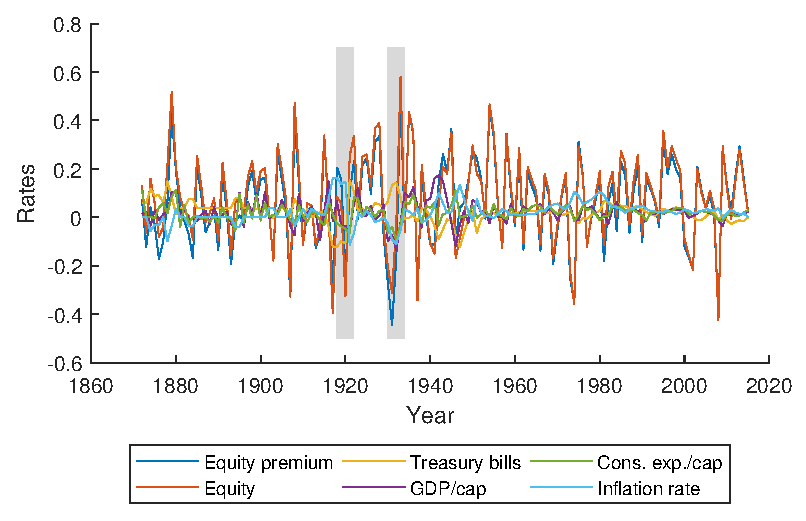
\includegraphics[width=\textwidth]{Matlab Graphics/Cons_disaster_US}
	\caption{US, consumption disasters}
	\label{fig:US_cons_disaster}
\end{figure}

For the US there were two disaster periods of equal lengths but different contraction sizes identified: the first one started 1918 with the onset of a global pandemic caused by an H1N1 virus, better known as the Spanish flu, which would later account for 500 million deaths worldwide and about 675,000 deaths occurring in the United States and triggered a depression in subsequent years lasting for four years (until 1922) with an average proportionate contraction of 18\%. The second consumption disaster period started in 1930 and captures the most severe part of the Great Depression where real consumption per capita fell about 23\% per year over this period (ended in 1934) (see \citet{Nakamura2013} for similar estimates).\\

The disaster probability $p$ is calculated as the total number of disasters (irrespective of duration) divided by the number of non-disaster years to provide a measure at an annual frequency. The expected disaster size $\mathop{\mathbb{E}}(b)$ is the unweighted average of annual proportionate declines > threshold.\\

{\renewcommand{\arraystretch}{1}
\begin{table}[H]
\begin{center}
\begin{tabular}{rccccc}
\hline
\hline
\multirow{3}{*}{Country} & \multirow{3}{*}{\shortstack{No.\\disasters}} & \multirow{3}{*}{\shortstack{No.\\disaster\\years}} & \multirow{3}{*}{\shortstack{No. non-\\disaster\\years}} & \multirow{3}{*}{\shortstack{Disaster\\probability\\(\%)}} & \multirow{3}{*}{\shortstack{Average\\disaster size\\(\%)}}\\
& & & & &\\
& & & & &\\
\hline
Australia & 6 & 17 & 128 & 4.69 & 22.60\\
Belgium$^{*}$ & 4 & 11 & 91 & 4.40 & 34.50\\
Denmark & 3 & 6 & 139 & 2.16 & 22.31\\
Finland & 5 & 16 & 129 & 3.90 & 21.75\\
France & 2 & 8 & 137 & 1.50 & 49.83\\
Germany & 4 & 17 & 128 & 3.13 & 31.75\\
Italy & 1 & 5 & 140 & 0.71 & 32.13\\
Japan$^{*}$ & 1 & 8 & 133 & 0.75 & 90.35\\
Netherlands & 3 & 10 & 135 & 2.22 & 42.14\\
Norway & 3 & 9 & 136 & 2.21 & 14.69\\
Portugal$^{*}$ & 3 & 9 & 96 & 3.13 & 15.25\\
Spain & 13 & 31 & 114 & 11.40 & 16.21\\
Sweden & 2 & 4 & 141 & 1.41 & 14.82\\
Switzerland & 6 & 14 & 131 & 4.60 & 17.73\\
United Kingdom & 2 & 8 & 137 & 1.50 & 17.72\\
United States & 2 & 8 & 137 & 1.50 & 20.02\\
\hline
$\Sigma$ & 60 & 181 & 2,052 & 2.92 & $\mu=28.99$\\
\hline
\hline
\multicolumn{6}{c}{$^{*}$ Belgium: 1914-2015, Japan: 1875-2015, Portugal: 1911-2015}
\end{tabular} 
\end{center}
\caption{Disaster risk moments (consumption)}
\label{tab:disaster_risk_consumption}
\end{table}

As table \ref{tab:disaster_risk_consumption} amd figure \ref{fig:Gant_consumption} show there is quite some variation across countries in propensity with respect to consumption disasters. 

\begin{figure}[H]
	\centering
  \includegraphics[width=\textwidth]{Graphics/Gantt_consumption_highres.PNG}
	\caption{Consumption disasters across countries over time}
	\label{fig:Gant_consumption}
\end{figure}

Clearly, wartime events affected most countries, though with different strength. Spain experienced multiple rather mild disasters whereas France, the Netherlands and Japan were hit by only few but abysmal events. The interactive version with additional information on individual disasters can be accessed from this \textcolor{blue}{\href{https://plotly.com/~gerwolf/54/consumption-disasters-percentage/}{link}}:\\
(https://plotly.com/~gerwolf/54/consumption-disasters-percentage/)
\\
Table \ref{tab:disaster_risk_gdp} and figure \ref{fig:Gant_GDP} in the appendix provide the same overview for GDP data. [\textcolor{blue}{\href{https://plotly.com/~gerwolf/68/gdp-disasters-percentage/}{Interactive version}}:\\
(https://plotly.com/~gerwolf/68/gdp-disasters-percentage/)]
\\
\\Consumption disasters occur slightly more frequently than GDP disasters but with a larger average contraction size. Notably, Japan suffered from the worst consumption disasters in the data set in the wake of WWII whereas the GDP contractions were not as severe. In general, average GDP contractions were less pronounced than consumption contractions which is probably due to the stabilizing measures taken by authorities by the onset of a disaster. Moreover, consumption tends to continue falling in response to a disaster shock before recovering, resulting in longer disaster durations pointing towards the crucial role of the IES and a high consumers' willingness to substitute consumption across time.






